\documentclass{article}
\usepackage[margin = 2.54cm]{geometry} % set margin to traditional doc

%packages
\usepackage{graphicx} % Required for inserting images
\usepackage[most]{tcolorbox} %for creating environments
\usepackage{amsmath}
\usepackage{amssymb}
\usepackage{mathtools}
\usepackage{verbatim}
\usepackage[utf8]{inputenc}
\usepackage[dvipsnames]{xcolor} %for importing multiple colors
\usepackage{hyperref} %for creating links to different sections

\linespread{1.2} %controlling line spread

%define colors i like
\definecolor{myTeal}{RGB}{0,128,128}
\definecolor{myGreen}{RGB}{34,170,34}
\definecolor{mySapphire}{RGB}{15,82,186}
\definecolor{myEmerald}{RGB}{50.4, 130, 90}

%create math environments, can add [section] or [subsection] to add index counter based on sections/subsections
\newtheorem{define}{Definition}
\newtheorem{prop}{Proposition}
\newtheorem{thm}{Theorem}
\newtheorem{question}{Question}
\newtheorem{lemma}{Lemma}

%setup colored box environment for each math env above
\tcolorboxenvironment{define}{
    enhanced, colframe=myTeal!50!teal, colback=myTeal!10,
    arc=5mm, lower separated=false, fonttitle=\bfseries, breakable
}
\tcolorboxenvironment{prop}{
    enhanced, colframe=myGreen!50!black, colback=myGreen!15,
    arc=5mm, lower separated=false, fonttitle=\bfseries, breakable
}
\tcolorboxenvironment{thm}{
    enhanced, colframe=mySapphire!50!mySapphire, colback=mySapphire!15,
    arc=5mm, lower separated=false, fonttitle=\bfseries, breakable
}
\tcolorboxenvironment{question}{
    enhanced, colframe=blue!50!black, colback=blue!10,
    arc=5mm, lower separated=false, fonttitle=\bfseries, breakable
}
\tcolorboxenvironment{lemma}{
    enhanced, colframe=myEmerald!50!myEmerald, colback=myEmerald!10,
    arc=5mm, lower separated=false, fonttitle=\bfseries, breakable
}

%setup hyperlink within pdf
\hypersetup{
    colorlinks=true,
    linkcolor=blue,
    filecolor=magenta,      
    urlcolor=cyan,
    pdftitle={Overleaf Example},
    pdfpagemode=FullScreen,
}

%common command (add to template)
%general
\newcommand{\FF}{\mathbb{F}}
\newcommand{\NN}{\mathbb{N}}
\newcommand{\ZZ}{\mathbb{Z}}
\newcommand{\QQ}{\mathbb{Q}}
\newcommand{\RR}{\mathbb{R}}
\newcommand{\CC}{\mathbb{C}}

\newcommand{\Id}{\textmd{Id}} %identity
\newcommand{\lcm}{\textmd{lcm}}
\DeclarePairedDelimiter{\abs}{\lvert}{\rvert}
\DeclarePairedDelimiter{\norm}{\lVert}{\rVert}
\DeclarePairedDelimiter{\paran}{(}{)}%paranthesis
\DeclarePairedDelimiter{\bracket}{\langle}{\rangle}

%algebra
\newcommand{\Gal}{\textmd{Gal}}
\newcommand{\Aut}{\textmd{Aut}}
\newcommand{\End}{\textmd{End}}
\newcommand{\Coker}{\textmd{Coker}}
\newcommand{\Hom}{\textmd{Hom}}
\newcommand{\Nil}{\textmd{Nil}}

%analysis
\newcommand{\Vol}{\textmd{Vol}}

%complex
\newcommand{\Real}{\textmd{Re}}
\newcommand{\Imag}{\textmd{Im}} %can also be used for Image
\newcommand{\Res}{\textmd{Res}}

%lie algebra
\newcommand{\gl}{\mathfrak{gl}}

\title{Phys 103 HW1 Pass 2}
\author{Zih-Yu Hsieh}

\begin{document}
\maketitle

\section*{Question 1}

\textbf{Pf:}

For this question, I didn't interpret the question right: \textbf{I didn't include the effect of the merry-go-round being frictionless, and thought the trajectory of the puck would rotate also at the same rate as the angular velocity of the merry-go-round.} 

On the other hand, I didn't notice that the traveling direction of the puck is toward the center, so I also need to adjust the radius function.

\hfil

Regardless of the case, if just consider the fact that the puck has velocity $v$ in negative radial direction (toward the center initially), with the initial radius $r(0)=R$, and the fact that the derivative of the radius function is $-v$ (since it is constantly going toward the center), we can construct the radius $r(t)=R-vt$.

(Note: If radius $r$ and angle $\phi$ can have the range of $\RR$, then the position of the puck can be expressed as continuous functions; if we limit radius to be nonnegative, there are cases where $\phi$ would instantly jump to $\pi+\phi$, causing the angle to be not continuous. If we want to verify that the velocity, i.e. derivative of position, is constantly $0$ or not, then we need the position to be differentiable. As long as $\phi$ is not continuous, taking derivative is invalid, so for mathematical rigor, assuming radius $r$ can be negative is more convenient).

\begin{figure}[h!]
    \begin{center}
        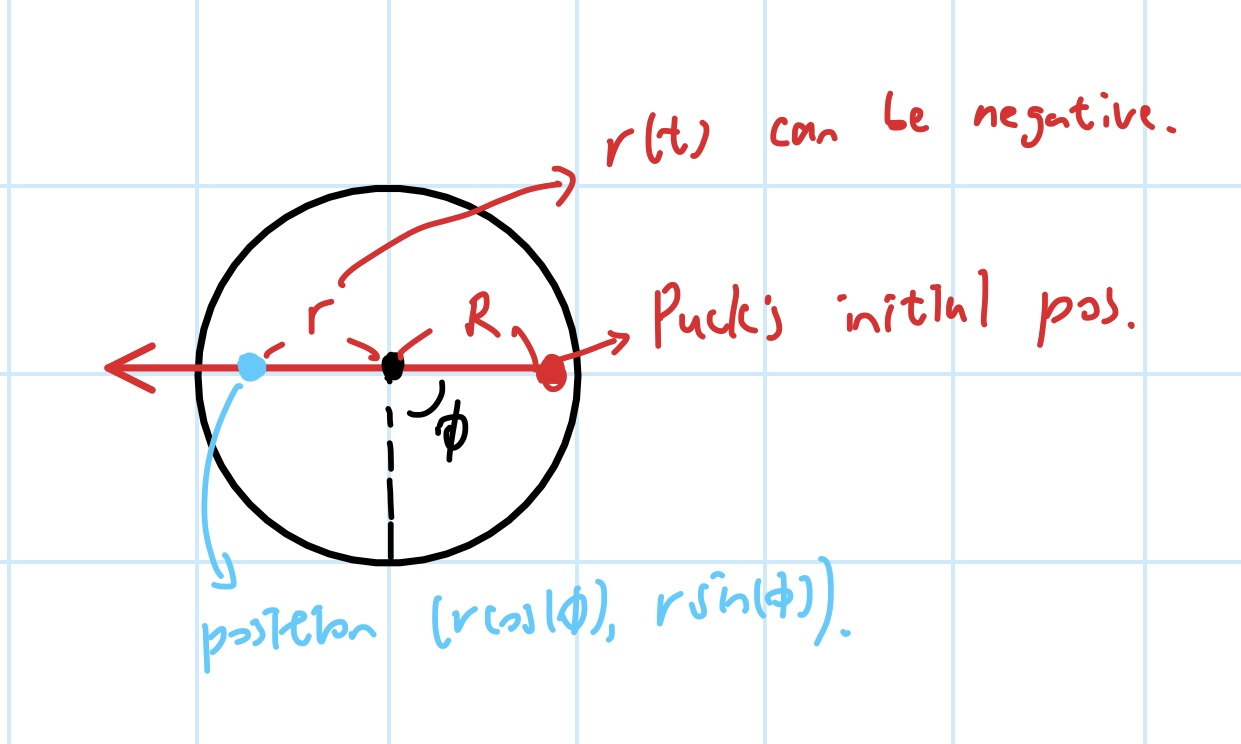
\includegraphics[width=100mm]{demonstration_q1.jpg}
        \caption{An illustraation of Position in $r$ and $\phi$}
    \end{center}
\end{figure}

\hfil

If the puck is not rotating with the merry-go-round, then here are the actual angles:

\subsection*{(a)}
Since the merry-go-round is frictionless, then the puck's angle wouldn't be affected by the merry-go-round (here, keep track of the puck's initial). And, since the observer is next to the merry-go-round (not rotating with it), the relative angle between the observer and the puck's initial position never changes. Which, if the angle $\phi$ records the puck's initial position's angle relative to the observer, we have $\phi(t)\cong 0$ (since the initial position never changes).

So, the puck's position is given by:
\begin{align}
    &\overline{x}(t)=(r\cos(\phi),r\sin(\phi)) = ((R-vt),0)\\
    &\implies\overline{a}= \ddot{\overline{x}} = \overline{0}
\end{align}
Since the acceleration is $\overline{0}$, then in this frame the puck (assumed to be an isolated object) is not accelerating, hence the observer is in an inertial frame.

\subsection*{(b)}
If the observer is constantly rotating with angular velocity $w$ (assuming it's counterclockwise), then to the observer, the puck's radius is still changing in the same way, so $r'(t) = R-vt$ again, while the puck's initial position is rotating with angular velocity $w$ in clockwise direction (or $-w$ in counterclockwise direction). With $\phi'(0)=0$. Then, we get that $\phi'(t) = -wt$ (since $\frac{d\phi'}{dt}=-w$, the angular velocity of the puck in the observer's frame).

So, the puck's position is given by:
\begin{align}
    &\overline{x'}(t)=(r'\cos(\phi'),r'\sin(\phi')) = (R-vt)(\cos(-wt),\sin(-wt)) = (R-vt)(\cos(wt),-\sin(wt))\\
    &\implies \overline{a'}(t)=\frac{d^2\overline{x'}}{dt^2} = (-2wv\sin(wt) - w^2(R+vt)\cos(wt), -2wv\cos(wt)+w^2(R+vt)\sin(wt))
\end{align}
Since the acceleration $\overline{a'}\neq \overline{0}$ in general, then the puck (the isolated object) is accelerating in this frame. Hence, the observer in (b) is not in an inertial frame.


\break

\section*{Question 2}


\textbf{Pf:}

In my original attempt, after doing massive calculation, I got to the part showing the following result:
\begin{equation}
    \sin^2(\theta)\approx \frac{1}{4}\paran*{1+\sqrt{1-\frac{4gh}{v_0^2}}}
\end{equation}
\textbf{However, in my final solution, I didn't use Taylor Series approximation to get an approximated results for $\theta$, which isn't the desired form of answer}.

As a result, for $\sqrt{1-x}$, its first derivative is given as follow:
\begin{equation}
    \frac{d}{dx}\sqrt{1-x}=-\frac{1}{2\sqrt{1-x}}
\end{equation}
Which, with the center about $x=0$, $\sqrt{1-x}\approx 1-\frac{1}{2}x$ when $x$ is small. Using this as a result, we get:
\begin{align}
    &\sin^2(\theta)\approx \frac{1}{4}\paran*{1+1-\frac{1}{2}\cdot \frac{4gh}{v_0^2}} = \frac{1}{2}-\frac{gh}{2v_0^2}\\
    &\implies \sin(\theta)\approx \frac{\sqrt{2}}{2}\sqrt{1-\frac{gh}{2v_0^2}}\approx \frac{\sqrt{2}}{2}\paran*{1-\frac{1}{2}\cdot\frac{gh}{v_0^2}} = \frac{\sqrt{2}}{2}\paran*{1-\frac{gh}{2v_0^2}}
\end{align}
Now, since we can assume $\theta$ is relatively close to $\frac{\pi}{4}$ (due to the fact that $h$ is small, so the maximum launch angle wouldn't be too far from $\frac{\pi}{4}$ - the solution corresponding to $h=0$), then we can do an taylor series approximation of $\sin(\theta)$ about $\theta = \frac{\pi}{4}$:

Since $\sin(\frac{\pi}{4})=\frac{\sqrt{2}}{2}$, and $(\sin(\theta))'\bigg|_{\theta=\frac{\pi}{4}} = \cos(\frac{\pi}{4})=\frac{\sqrt{2}}{2}$, we get $\sin(\theta)\approx \frac{\sqrt{2}}{2}+\frac{\sqrt{2}}{2}(\theta-\frac{\pi}{4})$ when $\theta\approx \frac{\pi}{4}$. Plug into the above equation, we get:
\begin{align}
    &\sin(\theta)\approx \frac{\sqrt{2}}{2}\paran*{1+\paran*{\theta-\frac{\pi}{4}}} \approx \frac{\sqrt{2}}{2}\paran*{1-\frac{gh}{2v_0^2}}\\
    &\implies 1+\paran*{\theta-\frac{\pi}{4}}\approx 1-\frac{gh}{2v_0^2}\\
    &\implies \theta\approx \frac{\pi}{4}-\frac{gh}{2v_0^2}
\end{align}
Which above is the desired form of approximation.


\break

\section*{Question 4}

\textbf{Pf:}

For this question, \textbf{even though the approximation of $\frac{r}{R}$ (with $r<<R$) is applied, but my final answer isn't in the approximation form up to linear term of $\frac{r}{R}$}, which is wrong in this context.

After lengthy calculation, the final answer is approximated as follow:
\begin{align}
    \Delta t&\approx \sqrt{\frac{R}{g}}\ln\left(\cot\left(\frac{r}{2R}\right)+\csc\left(\frac{r}{2R}\right)\right) = \sqrt{\frac{R}{g}}\ln\paran*{\frac{\cos(r/(2R))+1}{\sin(r/(2R))}}
\end{align}
With $\cos(x)\approx 1$ and $\sin(x)\approx x$ when $x$ is small, plug into the relation, we get:
\begin{align}
    \Delta t\approx \sqrt{\frac{R}{g}}\ln\paran*{\frac{1+1}{r/(2R)}} = \sqrt{\frac{R}{g}}\ln\paran*{\frac{4R}{r}}
\end{align}
This is the final form of approximation (in terms of natural log).

\hfil

\rule{15.6 cm}{0.1mm}

\hfil

As a side note, the previous comments of this question can be explained:

\begin{itemize}
    \item[1.] The first comment asking why choose $\cos(\theta)=\frac{1}{3}$, it's because here the purpose is to verify that the given term $4\cos(\theta)-6\cos^2(\theta)$ can be positive (if it's not positive, there's no way the inequality proposed could work, because then we would have $\frac{m}{M}$ bounded by some negative value, which is not possible with the masses being positive).
    \item[2.] The actual definition of infimum is as follow:
    \begin{define}
        Given a collection of real numbers $S\subseteq \RR$, the infimum of $S$ is defined as follow:
        $$m := \inf(S),\quad \textmd{for all }x \in S,\ m\leq x$$
        $$\textmd{For all } m'\in \RR,\ \textmd{such that every }x\in S\textmd{ satisfies }m'\leq x,\quad \textmd{it satisfies }m'\leq m$$
        In other words, $m$ is the "greatest lower bound" of the set of real numbers $S$.
    \end{define}
    Here, the infimum of $\frac{m}{M}$ means th greatest lower bound of $\frac{m}{M}$, which is the smallest number $\frac{m}{M}$ can be arbitrarily close to (it's just a more rigorous definition of what "infinitesimally small" in $\RR$ could be).
\end{itemize}

\break

\section*{Question 5}

\textbf{Pf:}

As of the first mistake, since here the propelled fuel has a speed of $u$ relative to the rocket, and propelled in the negative direction (for the rocket to go forward), then the actual relative velocity is $-u$. \textbf{So, the actual formula is in fact as below:}
\begin{align}
    \frac{dv}{dt}=-u\cdot\frac{1}{m}\frac{dm}{dt}-g
\end{align}
Since the original equation, the position of (-u) is the relative velocity of the propellant in the frame of the rocket. So, the solution of the velocity now becomes:
\begin{align}
    \Delta v&=\int_0^{\Delta t}\frac{dv}{dt}dt = \int_0^{\frac{m_f\cdot \tau}{m_e}}\left(-u\cdot\frac{1}{m}\frac{dm}{dt}-g\right)dt = -u\ln(m(t))\bigg|_0^{\Delta t}-g\Delta t\\
    &=-u\ln\left(\frac{m_{\textmd{fin}}}{m_0}\right)-\frac{g\cdot m_f\cdot \tau}{m_e} = -u\ln\left(\frac{m_t+m_e+m_p}{m_f+m_t+m_e+m_p}\right)-\frac{g\cdot m_f\cdot \tau}{m_e}\\
    &= u\ln\paran*{\frac{m_f+m_t+m_e+m_p}{m_t+m_e+m_p}}-\frac{g\cdot m_f\cdot \tau}{m_e}
\end{align}
The rest of the problems (when $u$ appears) need to add an extra negative sign.

\hfil

\rule{15.6cm}{0.1mm}

\hfil

As of the second mistake (calculation error),\textbf{my initial answer is $a_0\approx 0.0334-g$ (the first number in km/s$^2$; convert back in $g$ we get $a_0\approx 2.4g$ as my initial answer)}. Now, when calculating the initial acceleration given that $\tilde{m_p}=0.1$, I calculated $\tilde{m_e}\approx 0.0931$. And, the acceleration is given as follow:
\begin{align}
    \frac{dv}{dt}=-u\cdot \frac{1}{\tilde{m}}\frac{d\tilde{m}}{dt}-g = -u\cdot \frac{1}{\tilde{m}}\frac{-\tilde{m_e}}{\tau}-g = u\cdot\frac{\tilde{m_e}}{\tilde{m}\tau}-g
\end{align}
Which, with $u=3$km/s, $\tilde{m_e}= 0.0931$, $\tau=7$s, $\tilde{m_t}=1/10$, and $g=9.8$m/s, the initial acceleration is given as:
\begin{align}
    a_0 \approx 3\cdot \frac{0.0931}{7\cdot (1+0.1+0.0931+0.1)}-g \approx 0.0309-g
\end{align}
Where because of the unit of $u$, $0.0308561$ is in km/s$^2$; convert it back to m/s$^2$, we get:
\begin{align}
    a_0 \approx 30.856-g = 30.856-9.8 = 21.056 \approx 2.149 g
\end{align}
Which is close to the given answer $2.1g$ for $\tilde{m_p}=0.1$.

\break

\end{document}